\documentclass{article}

\usepackage{graphicx}
\usepackage{rotating}
\usepackage{mathtools}
\usepackage{wrapfig}

\DeclarePairedDelimiter{\ceil}{\lceil}{\rceil}
\DeclarePairedDelimiter{\floor}{\lfloor}{\rfloor}
\title{Obstacle Avoiding Mobile Vehicle with Rewind}
\author{Jonathan A. Garcia-Mallen}
\date{31 October 2017}

\begin{document}
\maketitle

% Is the overview just the abstract? Because that's what it is right now. 
\section*{Overview} 
% copied from abstract.md
The goal is to have a robot go forward and avoid any obstacles in the way. After a certain period of time has passed, the robot will stop. Then a button can be pressed to initiate rewind. When the robot rewinds, it returns to its start pose via the same path it used to reach its end pose. Any turns it makes on the forward trip are done in reverse for the return trip. While rewinding, it performs no obstacle avoidance. To avoid obstacles, three to five ultrasonic sensors, or three to five IR emitters paired with IR receivers can used as rangefinders. The robot itself is supplied by the student.   


\begin{wrapfigure}{r}{.4\textwidth}
  \centering
  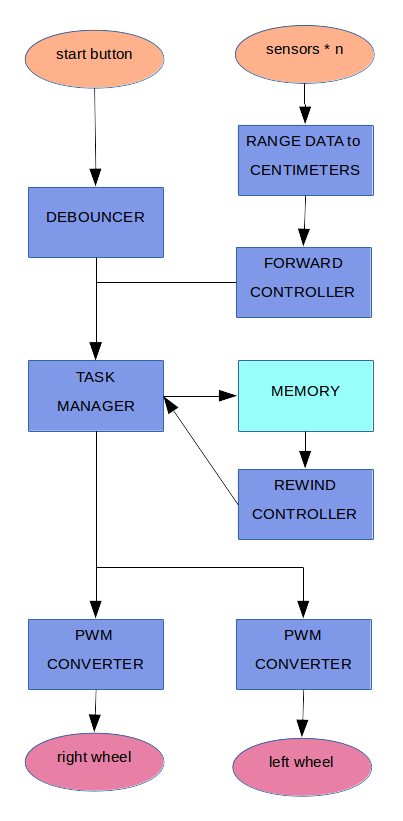
\includegraphics[width=.4\textwidth]{block_diagram.png}
\end{wrapfigure}

\section*{System Architecture} 
The task manager coordinates the system. It receives the start signal from the start button and passes wheel commands from the controllers to the PWM modules. 
The forward controller receives sensor data and calculates wheel commands to send to the task manager. 
The rewind controller pulls the commands from memory, reverses them, and sends wheel commands such that the robot traverses the path it just followed, but in reverse. 
The memory itself will likely be BRAM, and will store a subset of the wheel commands received by the task manager from the forward controller. The sample rate will also be stored. 
PWM converter is a module; we will have a left instance and a right instance. They take wheel commands from the task manager and convert them to waves to control the servo motors. 

% For each subsection: 
%   inputs
%   outputs
%   what it does / its purpose
\subsection*{System Inputs and Outputs}
Start button starts. 
We have n sensors, where n can go from three to five. The sensors are IR range sensors. 

\subsection*{Forward Controller}
This takes input from the raw\_to\_dist module, which will do cleanup on the sensors. It receives raw data as input and outputs clean range data in centimeters. Clean data is data that does not jump around. If multipath issues with the IR sensors, raw\_to\_dist cleans them away. raw\_to\_dist will be instantiated n times in the forward controller, once for each IR sensor. 

The forward controller receives this clean sensor data as input. It is a simple proportional controller. The sensors on the right side of the robot push the robot away from obstacles on the right; sensors on the left push the vehicle away from obstacles on the left. This is done with the following calculation: 
\begin{equation}
wheel\_l = speed * (\sum_{i=0}^{\floor{n/2}}{p_ir_i}) \end{equation}
\begin{equation}wheel\_r = speed * (\sum_{i=\ceil{n/2}}^{n}{p_ir_i})
\end{equation}
The value $r_i$ is the clean sensor data. The values speed and $p_i$ are parameters passed into the forward controller module. Both wheel values range from zero to 127, and are 7-bit wires. Note that the vehicle only ever moves forward. We will make no fast turns. 

\subsection*{Rewind Controller and Memory}
% write about memory
The rewind controller pulls the wheel commands from memory. The same commands sent to the same wheels and scaled by $-1$ suffices to rewind the robot. However, the rewind controller must upsample the commands by the sample rate. Investigation is also re
\subsection*{PWM Converter and System Outputs}
\subsection*{Task Manager} 
The task manager runs a small three-state finite state machine. The robot is in either IDLE, FORWARD, or REWIND states. The most important parameter it receives is the time of the run. This may be determined by the switches on the Nexys 4, but will initially be set at ten seconds.  

The system transitions from IDLE to FORWARD when the task manager receives the debounced start signal from the button. This module then sends a forward\_enable signal to the forward controller to begin receiving wheel commands. These commands are downsampled and saved into the memory. 

\section*{Complexity Analysis}

\section*{Bill of Materials}
The components required are listed below, and the vehicle in its current state is pictured. 

\begin{itemize}
  \item wheels and chassis
  \item battery pack
  \item SpringRC SM-S4303R Continuous Rotation Servos, operable at 4.8 Volts [1].
  \item IR sensors
  \item Nexys 4 
\end{itemize}
\begin{turn}{180} 
  % system photo viewer sees an upright photo. Latex doesn't. 
  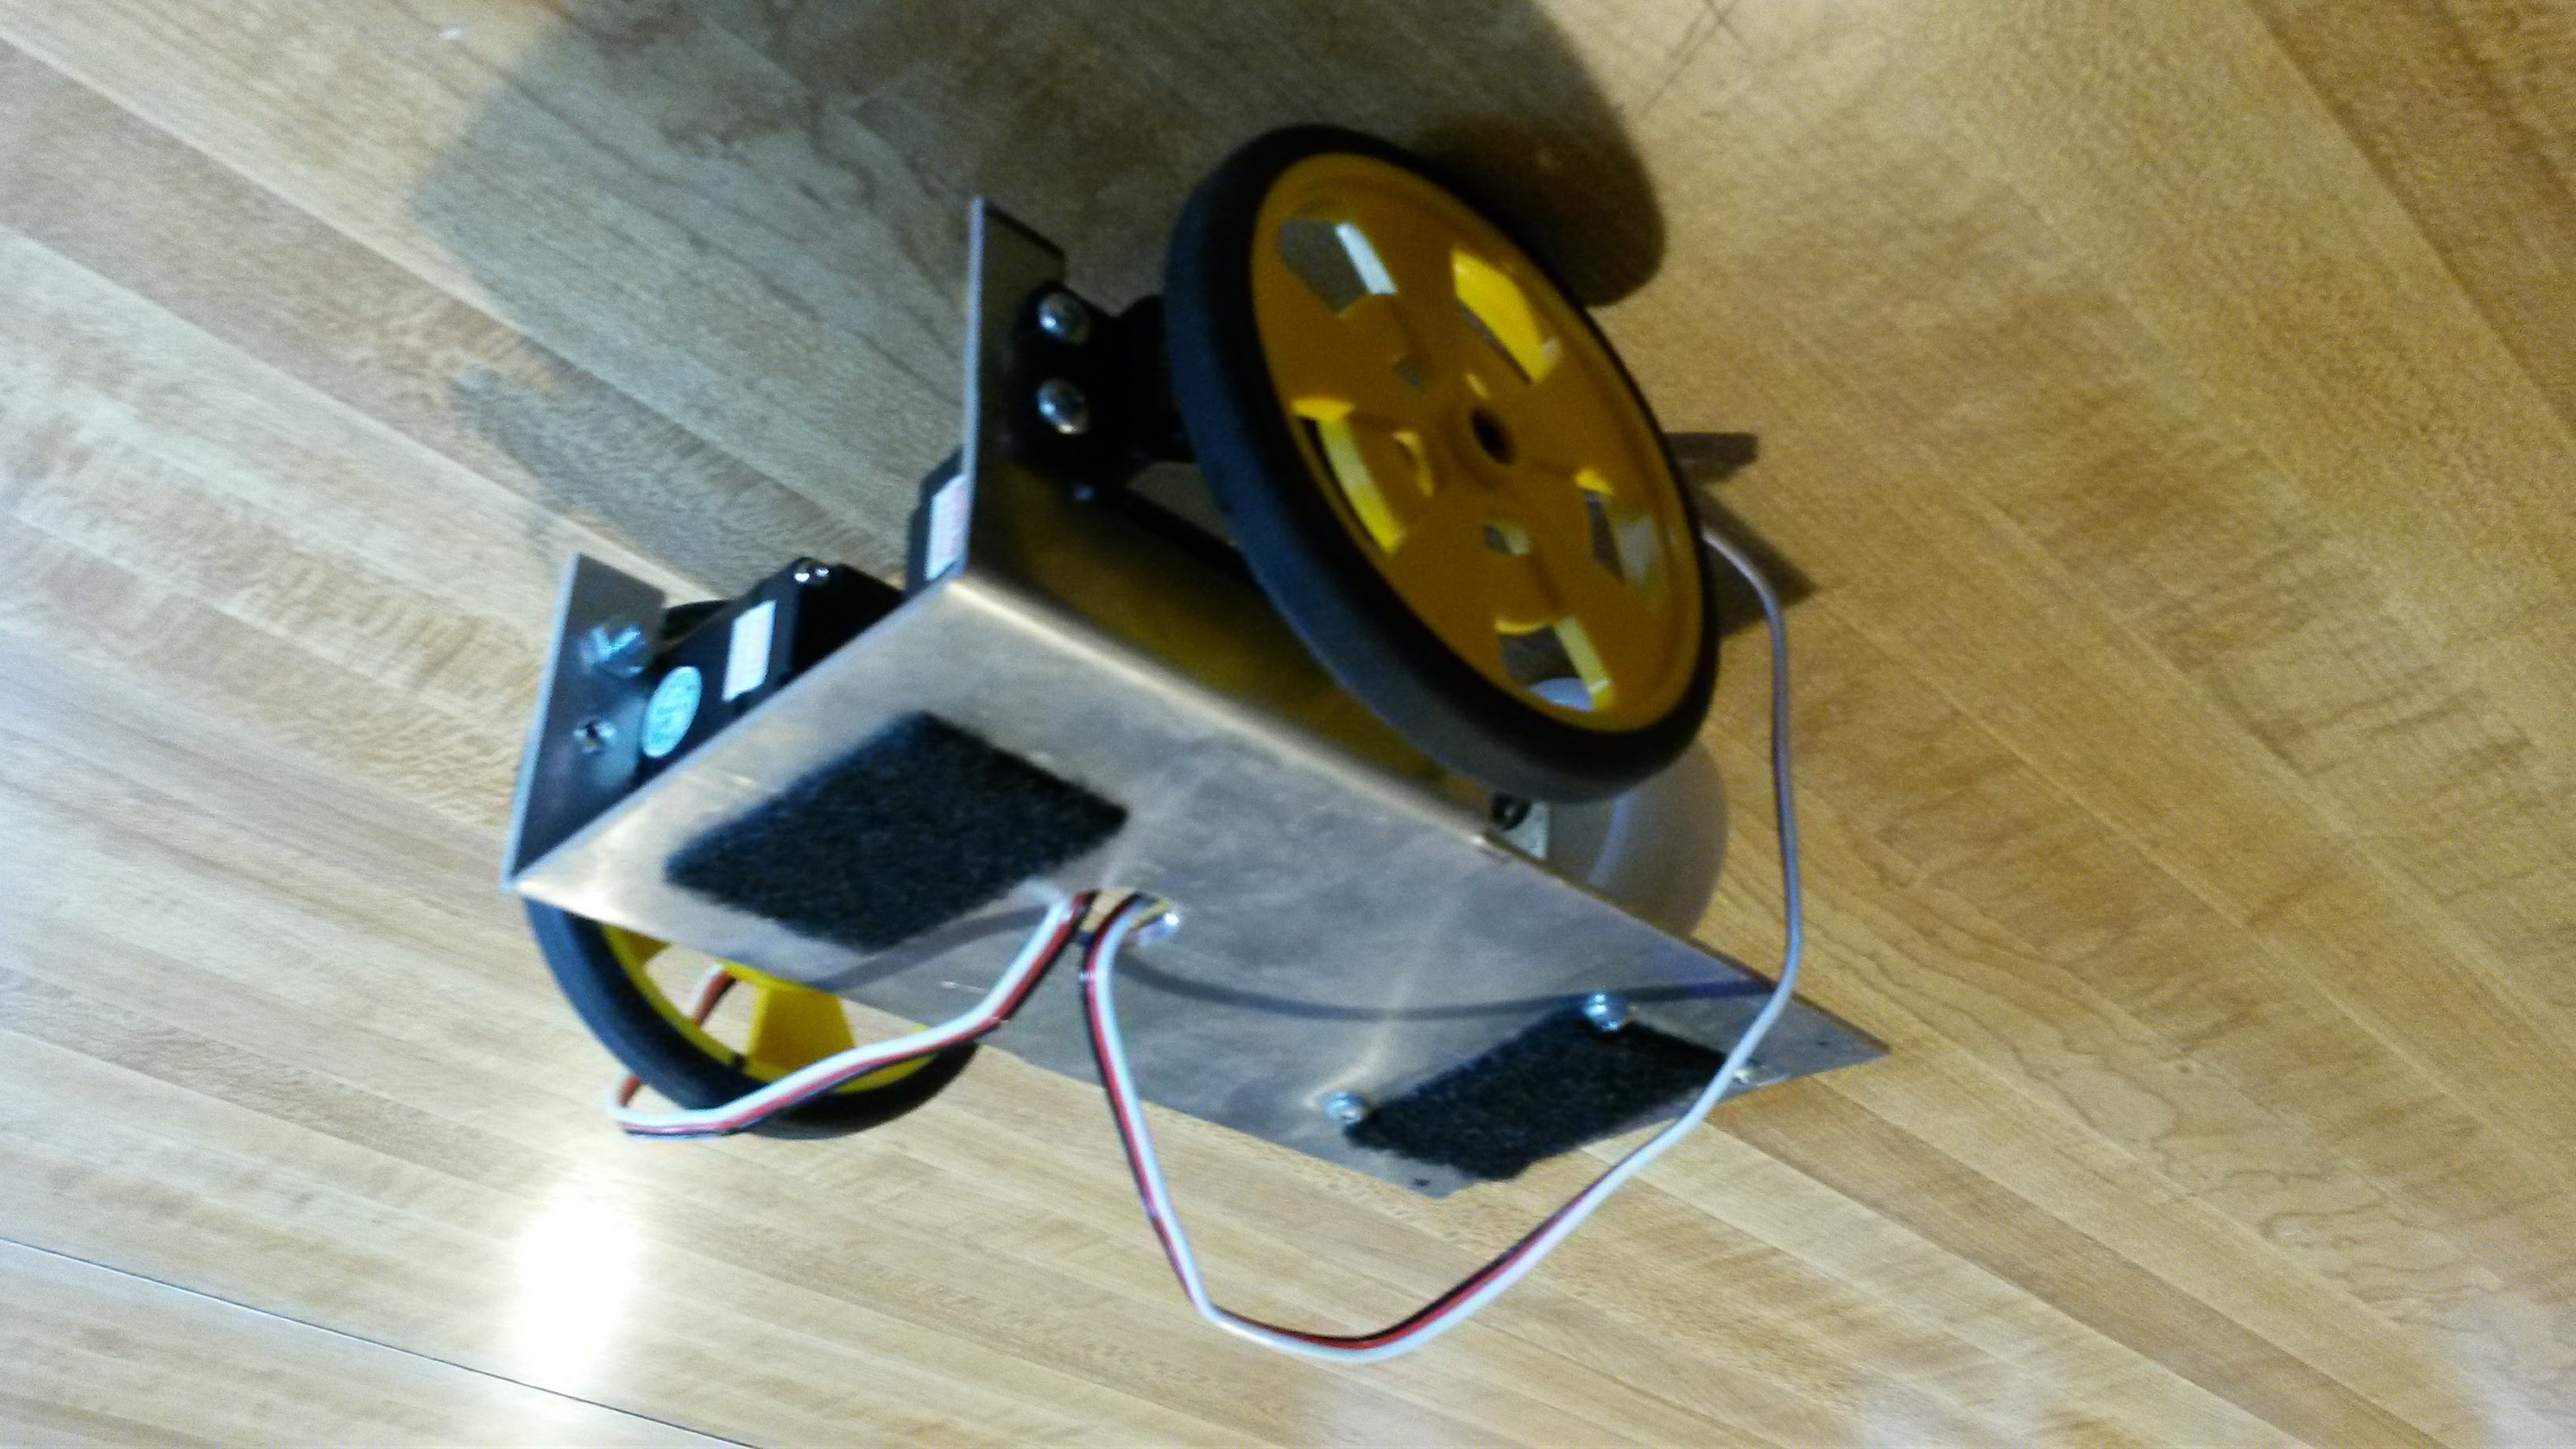
\includegraphics[width=\textwidth]{chassis.jpg}
\end{turn}

\section*{Timeline}

\section*{References}
\begin{enumerate}
  \item https://www.pololu.com/product/1248/specs
\end{enumerate}

\end{document}

